\graphicspath{{./img/}}
\section{Đề số 4}

\begin{bt} 
   \hfill
   \begin{enumerate}[a.]
    \item Thực hiện phép tính: $\mathrm{A}=\left[\left(\frac{2}{193}-\frac{3}{386}\right) \cdot \frac{193}{17}+\frac{33}{34}\right]:\left[\left(\frac{7}{1931}+\frac{11}{3862}\right) \cdot \frac{1931}{25}+\frac{9}{2}\right]$.
    \item Rút gọn :    
    $$
    \mathrm{B}=(-5)^0+(-5)^1+(-5)^2+(-5)^3+\ldots+(-5)^{2016}+(-5)^{2017}
    $$
   \end{enumerate}
\loigiai{} 
\end{bt}

\begin{bt}
    \hfill
    \begin{enumerate}[a.]
        \item Tìm a, b, c biết $\quad \frac{12 a-15 b}{7}=\frac{20 c-12 a}{9}=\frac{15 b-20 c}{11}$ và $a+b+c=48$.
        \item Một công trường dự định phân chia số đất cho ba đội I, II, III tỉ lệ với 7; 6; 5 . Nhưng sau đó vì số người của các đội thay đổi nên đã chia lại tỉ lệ với $6 ; 5 ; 4$. Như vậy có một đội làm nhiều hơn so với dự định là $6 \mathrm{m}^3$ đất. Tính tổng số đất đã phân chia cho các đội.
    \end{enumerate}
\loigiai{} 
\end{bt}

\begin{bt}
   \hfill
   \begin{enumerate}[a.]
    \item Tìm giá trị nhỏ nhất của biểu thức: $C=\frac{|x-2017|+2018}{|x-2017|+2019}$.
    \item Chứng tỏ rằng $\mathrm{S}=\frac{3}{4}+\frac{8}{9}+\frac{15}{16}+\ldots+\frac{\mathrm{n}^2-1}{\mathrm{n}^2}$ không là số tự nhiên với mọi $\mathrm{n} \in \mathrm{N}, \mathrm{n}>$2.
    \item Tìm tất cả các cặp số nguyên $x$, $y$ sao cho: $x-2 x y+y=0$.
   \end{enumerate}
\loigiai{} 
\end{bt}

\begin{bt}
    Cho tam giác cân $A B C, A B=A C$. Trên cạnh $B C$ lấy điểm $D$, trên tia đối của $C B$ lấy điểm $\mathrm{E}$ sao cho $\mathrm{BD}=\mathrm{CE}$. Các đường thẳng vuông góc với $\mathrm{BC}$ kẻ từ $\mathrm{D}$ và $\mathrm{E}$ cắt $\mathrm{AB}$ và $A C$ lân lượt ở $M$ và $N$. Chứng minh rằng: 
    \begin{enumerate}[a.]
    \item $\mathrm{DM}=\mathrm{EN}$.
    \item Đường thẳng $\mathrm{BC}$ cắt $\mathrm{MN}$ tại điểm $\mathrm{I}$ là trung điểm của $\mathrm{MN}$.
    \item Đường thẳng vuông góc với $\mathrm{MN}$ tại I luôn luôn đi qua một điểm cố định khi $\mathrm{D}$ thay đổi trên cạnh BC.
    \end{enumerate}
\loigiai{}
\end{bt}

\begin{bt}
    \begin{wrapfigure}{r}{0.35\textwidth}
        \centering
        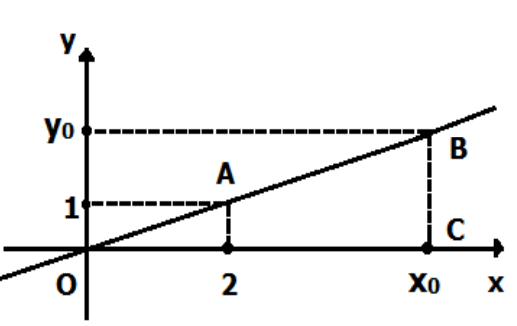
\includegraphics[width=0.35\textwidth]{ds4-b5.png}
    \end{wrapfigure}
    Trong hình bên, đường thẳng $\mathrm{OA}$ là đồ thị của hàm số $\mathrm{y}=\mathrm{f}(\mathrm{x})=\mathrm{ax}$.
    \begin{enumerate}[a.]
        \item  Tính tỉ số $\frac{\mathrm{y}_0-2}{\mathrm{x}_0-4}$.
        \item Giả sử $x_0=5$. Tính diện tích tam giác $\mathrm{OBC}$
    \end{enumerate}
    \loigiai{}
\end{bt}